\documentclass{ximera}
 

\usepackage{epsfig}

\graphicspath{
  {./}
  {figures/}
}

\usepackage{morewrites}
\makeatletter
\newcommand\subfile[1]{%
\renewcommand{\input}[1]{}%
\begingroup\skip@preamble\otherinput{#1}\endgroup\par\vspace{\topsep}
\let\input\otherinput}
\makeatother

\newcommand{\includeexercises}{\directlua{dofile("/home/jim/linearAlgebra/laode/exercises.lua")}}

%\newcounter{ccounter}
%\setcounter{ccounter}{1}
%\newcommand{\Chapter}[1]{\setcounter{chapter}{\arabic{ccounter}}\chapter{#1}\addtocounter{ccounter}{1}}

%\newcommand{\section}[1]{\section{#1}\setcounter{thm}{0}\setcounter{equation}{0}}

%\renewcommand{\theequation}{\arabic{chapter}.\arabic{section}.\arabic{equation}}
%\renewcommand{\thefigure}{\arabic{chapter}.\arabic{figure}}
%\renewcommand{\thetable}{\arabic{chapter}.\arabic{table}}

%\newcommand{\Sec}[2]{\section{#1}\markright{\arabic{ccounter}.\arabic{section}.#2}\setcounter{equation}{0}\setcounter{thm}{0}\setcounter{figure}{0}}

\newcommand{\Sec}[2]{\section{#1}}

\setcounter{secnumdepth}{2}
%\setcounter{secnumdepth}{1} 

%\newcounter{THM}
%\renewcommand{\theTHM}{\arabic{chapter}.\arabic{section}}

\newcommand{\trademark}{{R\!\!\!\!\!\bigcirc}}
%\newtheorem{exercise}{}

\newcommand{\dfield}{{\sf dfield9}}
\newcommand{\pplane}{{\sf pplane9}}

\newcommand{\EXER}{\section*{Exercises}}%\vspace*{0.2in}\hrule\small\setcounter{exercise}{0}}
\newcommand{\CEXER}{}%\vspace{0.08in}\begin{center}Computer Exercises\end{center}}
\newcommand{\TEXER}{} %\vspace{0.08in}\begin{center}Hand Exercises\end{center}}
\newcommand{\AEXER}{} %\vspace{0.08in}\begin{center}Hand Exercises\end{center}}

% BADBAD: \newcommand{\Bbb}{\bf}

\newcommand{\R}{\mbox{$\Bbb{R}$}}
\newcommand{\C}{\mbox{$\Bbb{C}$}}
\newcommand{\Z}{\mbox{$\Bbb{Z}$}}
\newcommand{\N}{\mbox{$\Bbb{N}$}}
\newcommand{\D}{\mbox{{\bf D}}}
\usepackage{amssymb}
%\newcommand{\qed}{\hfill\mbox{\raggedright$\square$} \vspace{1ex}}
%\newcommand{\proof}{\noindent {\bf Proof:} \hspace{0.1in}}

\newcommand{\setmin}{\;\mbox{--}\;}
\newcommand{\Matlab}{{M\small{AT\-LAB}} }
\newcommand{\Matlabp}{{M\small{AT\-LAB}}}
\newcommand{\computer}{\Matlab Instructions}
\newcommand{\half}{\mbox{$\frac{1}{2}$}}
\newcommand{\compose}{\raisebox{.15ex}{\mbox{{\scriptsize$\circ$}}}}
\newcommand{\AND}{\quad\mbox{and}\quad}
\newcommand{\vect}[2]{\left(\begin{array}{c} #1_1 \\ \vdots \\
 #1_{#2}\end{array}\right)}
\newcommand{\mattwo}[4]{\left(\begin{array}{rr} #1 & #2\\ #3
&#4\end{array}\right)}
\newcommand{\mattwoc}[4]{\left(\begin{array}{cc} #1 & #2\\ #3
&#4\end{array}\right)}
\newcommand{\vectwo}[2]{\left(\begin{array}{r} #1 \\ #2\end{array}\right)}
\newcommand{\vectwoc}[2]{\left(\begin{array}{c} #1 \\ #2\end{array}\right)}

\newcommand{\ignore}[1]{}


\newcommand{\inv}{^{-1}}
\newcommand{\CC}{{\cal C}}
\newcommand{\CCone}{\CC^1}
\newcommand{\Span}{{\rm span}}
\newcommand{\rank}{{\rm rank}}
\newcommand{\trace}{{\rm tr}}
\newcommand{\RE}{{\rm Re}}
\newcommand{\IM}{{\rm Im}}
\newcommand{\nulls}{{\rm null\;space}}

\newcommand{\dps}{\displaystyle}
\newcommand{\arraystart}{\renewcommand{\arraystretch}{1.8}}
\newcommand{\arrayfinish}{\renewcommand{\arraystretch}{1.2}}
\newcommand{\Start}[1]{\vspace{0.08in}\noindent {\bf Section~\ref{#1}}}
\newcommand{\exer}[1]{\noindent {\bf \ref{#1}}}
\newcommand{\ans}{}
\newcommand{\matthree}[9]{\left(\begin{array}{rrr} #1 & #2 & #3 \\ #4 & #5 & #6
\\ #7 & #8 & #9\end{array}\right)}
\newcommand{\cvectwo}[2]{\left(\begin{array}{c} #1 \\ #2\end{array}\right)}
\newcommand{\cmatthree}[9]{\left(\begin{array}{ccc} #1 & #2 & #3 \\ #4 & #5 &
#6 \\ #7 & #8 & #9\end{array}\right)}
\newcommand{\vecthree}[3]{\left(\begin{array}{r} #1 \\ #2 \\
#3\end{array}\right)}
\newcommand{\cvecthree}[3]{\left(\begin{array}{c} #1 \\ #2 \\
#3\end{array}\right)}
\newcommand{\cmattwo}[4]{\left(\begin{array}{cc} #1 & #2\\ #3
&#4\end{array}\right)}

\newcommand{\Matrix}[1]{\ensuremath{\left(\begin{array}{rrrrrrrrrrrrrrrrrr} #1 \end{array}\right)}}

\newcommand{\Matrixc}[1]{\ensuremath{\left(\begin{array}{cccccccccccc} #1 \end{array}\right)}}



\renewcommand{\labelenumi}{\theenumi)}
\newenvironment{enumeratea}%
{\begingroup
 \renewcommand{\theenumi}{\alph{enumi}}
 \renewcommand{\labelenumi}{(\theenumi)}
 \begin{enumerate}}
 {\end{enumerate}\endgroup}



\newcounter{help}
\renewcommand{\thehelp}{\thesection.\arabic{equation}}

%\newenvironment{equation*}%
%{\renewcommand\endequation{\eqno (\theequation)* $$}%
%   \begin{equation}}%
%   {\end{equation}\renewcommand\endequation{\eqno \@eqnnum
%$$\global\@ignoretrue}}

%\input{psfig.tex}

\author{Martin Golubitsky and Michael Dellnitz}

%\newenvironment{matlabEquation}%
%{\renewcommand\endequation{\eqno (\theequation*) $$}%
%   \begin{equation}}%
%   {\end{equation}\renewcommand\endequation{\eqno \@eqnnum
% $$\global\@ignoretrue}}

\newcommand{\soln}{\textbf{Solution:} }
\newcommand{\exercap}[1]{\centerline{Figure~\ref{#1}}}
\newcommand{\exercaptwo}[1]{\centerline{Figure~\ref{#1}a\hspace{2.1in}
Figure~\ref{#1}b}}
\newcommand{\exercapthree}[1]{\centerline{Figure~\ref{#1}a\hspace{1.2in}
Figure~\ref{#1}b\hspace{1.2in}Figure~\ref{#1}c}}
\newcommand{\para}{\hspace{0.4in}}

\renewenvironment{solution}{\suppress}{\endsuppress}

\ifxake
\newenvironment{matlabEquation}{\begin{equation}}{\end{equation}}
\else
\newenvironment{matlabEquation}%
{\let\oldtheequation\theequation\renewcommand{\theequation}{\oldtheequation*}\begin{equation}}%
  {\end{equation}\let\theequation\oldtheequation}
\fi

\makeatother

\begin{document}

\noindent In Exercises~\ref{c4.10A.4a} -- \ref{c4.10A.4b}, find the solution 
to $\dot{X} = CX$ satisfying $X(0)=X_0$ in two different ways, as follows.  
\begin{itemize}
\item[(a)]  Use {\pplane} to find $X(0.5)$.  {\bf Hint}: Use the 
{\sf Specify a computation interval} option in the {\sf PPLANE9 Keyboard input} 
window to compute the solution to $t=0.5$. Then use the {\sf zoom in square} 
feature to determine an answer to three decimal places.  
\item[(b)]  Next use \Matlab to find the eigenvalues and eigenvectors of $C$ 
and to find a closed form solution $X(t)$.  Use this formula to evaluate 
$X(0.5)$ to three decimal places.    
\item[(c)]  Do the two answers agree?
\end{itemize}
\begin{computerExercise}  \label{c4.10A.4a}  
$C = \mattwo{2.65}{-2.34}{-1.5}{-1.2} \AND X_0=\vectwo{0.5}{0.1}$.

\begin{solution}
\ans $X(0.5) = (0.155,0.386)^t$ and the two methods agree to three 
decimal places.

\soln (a) The result of the {\sf pplane5} integration is given in 
Figure~\ref{c4.10A.4a}a. After zooming several times we arrive at
Figure~\ref{c4.10A.4a}b.  By inspection $X(0.5)=(0.155,0.386)$.

(b)  Enter the matrix $C$ into \Matlab by typing
\begin{verbatim}
C = [2.65 -2.34; -1.5 -1.2];
\end{verbatim}
Find the eigenvalues and eigenvectors of this matrix by typing {\tt [V,D] = eig(C)}
and obtaining
\begin{verbatim}
V =
    0.9510    0.4525
   -0.3093    0.8918
D =
    3.4112         0
         0   -1.9612
\end{verbatim}
Therefore the general solution to this differential equation is:
\[
X(t) = \alpha e^{3.4112 t}\vectwo{0.9510}{-0.3093} +
\beta e^{-1.9612 t}\vectwo{0.4525}{0.8918}.
\]
It follows that 
\[
X(0) = V \vectwo{\alpha}{\beta}
\]
Therefore,
\[
\vectwo{\alpha}{\beta} = V\inv X_0 = 
\mattwo{0.9510}{0.4525}{-0.3093}{0.8918}\vectwo{0.5}{1.0} = \vectwo{-0.0067}{1.1191}
\]
The last calculation is done by typing {\tt coeff = inv(V)*[0.5;1.0]}. 
Therefore, the solution to the initial value problem is:
\[
X(t) = -0.0067e^{3.4112 t}\vectwo{0.9510}{-0.3093} +
1.1191e^{-1.9612 t}\vectwo{0.4525}{0.8918}.
\]
We can evaluate $X(0.5)$ in \Matlab by typing
\begin{verbatim}
X5 = coeff(1)*exp(D(1,1)*0.5)*V(:,1) + coeff(2)*exp(D(2,2)*0.5)*V(:,2)
\end{verbatim}
and obtaining
\begin{verbatim}
X5 =
    0.1547
    0.3858
\end{verbatim}


(c)  The two answers agree to three decimal places.

\begin{figure}[htb]
                       \centerline{%
                       \psfig{file=exfigure/4-9-8a.eps,width=2.75in}
                       \psfig{file=exfigure/4-9-8b.eps,width=2.75in}}
                \exercaptwo{c4.10A.4a}
\end{figure}



\end{solution}
\end{computerExercise}
\begin{computerExercise}  \label{c4.10A.4b}  
$C = \mattwo{1.2}{2.4}{0.6}{-3.5} \AND X_0=\vectwo{0.5}{0.7}$.

\begin{solution}
\ans $X(0.5) = (1.621,0.291)^t$ and the two methods agree to three 
decimal places.

\soln (a) The result of the {\sf pplane5} integration is given in 
Figure~\ref{c4.10A.4b}a. After zooming several times we arrive at
Figure~\ref{c4.10A.4b}b.  By inspection $X(0.5)=(1.621,0.291)$.

(b) (b)  Enter the matrix $C$ into \Matlab by typing
\begin{verbatim}
C = [1.2 2.4; 0.6 -3.5];
\end{verbatim}
Find the eigenvalues and eigenvectors of this matrix by typing {\tt [V,D] = eig(C)}
and obtaining
\begin{verbatim}
V =
    0.9928   -0.4335
    0.1194    0.9011
D =
    1.4887         0
         0   -3.7887
\end{verbatim}
Therefore the general solution to this differential equation is:
\[
X(t) = \alpha e^{1.4887 t}\vectwo{0.9928}{0.1194} +
\beta e^{-3.7887 t}\vectwo{-0.4335}{0.9011}.
\]
It follows that 
\[
X(0) = V \vectwo{\alpha}{\beta}
\]
Therefore,
\[
\vectwo{\alpha}{\beta} = V\inv X_0 = 
\mattwo{0.9928}{-0.4335}{0.1194}{0.9011}\vectwo{0.5}{0.7} = \vectwo{0.7967}{0.6712}
\]
The last calculation is done by typing {\tt coeff = inv(V)*[0.5;0.7]}. 
Therefore, the solution to the initial value problem is:
\[
X(t) = 0.7967e^{1.4887 t}\vectwo{0.9928}{0.1194} +
0.6712e^{-3.7887 t}\vectwo{-0.4335}{0.9011}.
\]
We can evaluate $X(0.5)$ in \Matlab by typing
\begin{verbatim}
X5 = coeff(1)*exp(D(1,1)*0.5)*V(:,1) + coeff(2)*exp(D(2,2)*0.5)*V(:,2)
\end{verbatim}
and obtaining
\begin{verbatim}
X5 =
    1.6213
    0.2912
\end{verbatim}

(c)  The two answers agree to three decimal places.


\begin{figure}[htb]
                       \centerline{%
                       \psfig{file=exfigure/4-9-9a.eps,width=2.75in}
                       \psfig{file=exfigure/4-9-9b.eps,width=2.75in}}
                \exercaptwo{c4.10A.4b}
\end{figure}



\end{solution}
\end{computerExercise}
\end{document}
